\documentclass{article}
\title{CSC301 HW9}
\author{Alex Zhang}
\date{April 2023}
\textwidth=16.00cm 
\textheight=22.00cm 
\topmargin=0.00cm
\oddsidemargin=0.00cm 
\evensidemargin=0.00cm 
\headheight=0cm 
\headsep=0.5cm
\textheight=610pt
\usepackage{graphicx}
\usepackage{multicol}




\graphicspath{ {./images/} }

\usepackage{latexsym,array,delarray,amsthm,amssymb,epsfig}
\usepackage{amsmath}
\usepackage{listings}
\lstset{
  basicstyle=\ttfamily,
  mathescape
}


\newcommand{\bmat}[1]{\begin{bmatrix} #1 \end{bmatrix}}
\newcommand{\mat}[1]{\mathbf{#1}}

\let\ds\displaystyle

\begin{document}
\maketitle

\section*{Question 1}

The pseudocode for PAR-MATMUL algorithm is below,
\begin{multicols}{2}
  \begin{lstlisting}
    function PAR-MATMUL(A,B)
      parallel for i = 1 to n do
        parallel for j = 1 to n do
          $C_{ij}$ = DOT($A_i$,$B_j$)
        end for
      end for
    end function
  \end{lstlisting}
  \begin{lstlisting}
    fucntion d = DOT(x,y)
      if n = 1 then
        return $\mat{x} \cdot \mat{y}$
      $\mat{x} = [\mat{x}_L \text{ }\mat{x}_R] $, $\mat{y} = [\mat{y}_L \text{ } \mat{y}_R]$
      spawn $d_L =$ DOT($\mat{x}_L \text{ } \mat{y}_L$)
            $d_R =$ DOT($\mat{x}_R \text{ } \mat{y}_R$)
      sync 
      return $d_L + d_R$ 
  \end{lstlisting}
\end{multicols} 
\paragraph{Costs Analysis} Time\\

For DOT function, it's work recurrence is 
$$T_1(n) = 2T_1(n/2) + O(1)$$
and span recurrence is 
$$T_{\infty}(n) = T_{\infty}(n/2) + O(1)$$
Using master theorem, $T_1(n) = O(n)$, $T_{\infty}(n) = O(\log n)$.


For PAR-MATMUL function, it's work costs is 
$$T_1(n) = O(n^3)$$

It's span costs $$O(\log n) + O(\log n) + O(\log n)$$
which contains two parallel loops and a parallel recursion dot product.
So it's span will be $O(3\log n) = O(\log n)$.



Overall, This parallel algorithm for matrix multiplication will have $O(n^3)$ work and $O(\log n)$ span.

\section*{Question 2}
Based on the recurrence, I can draw the following substitution graph:
\begin{center}
    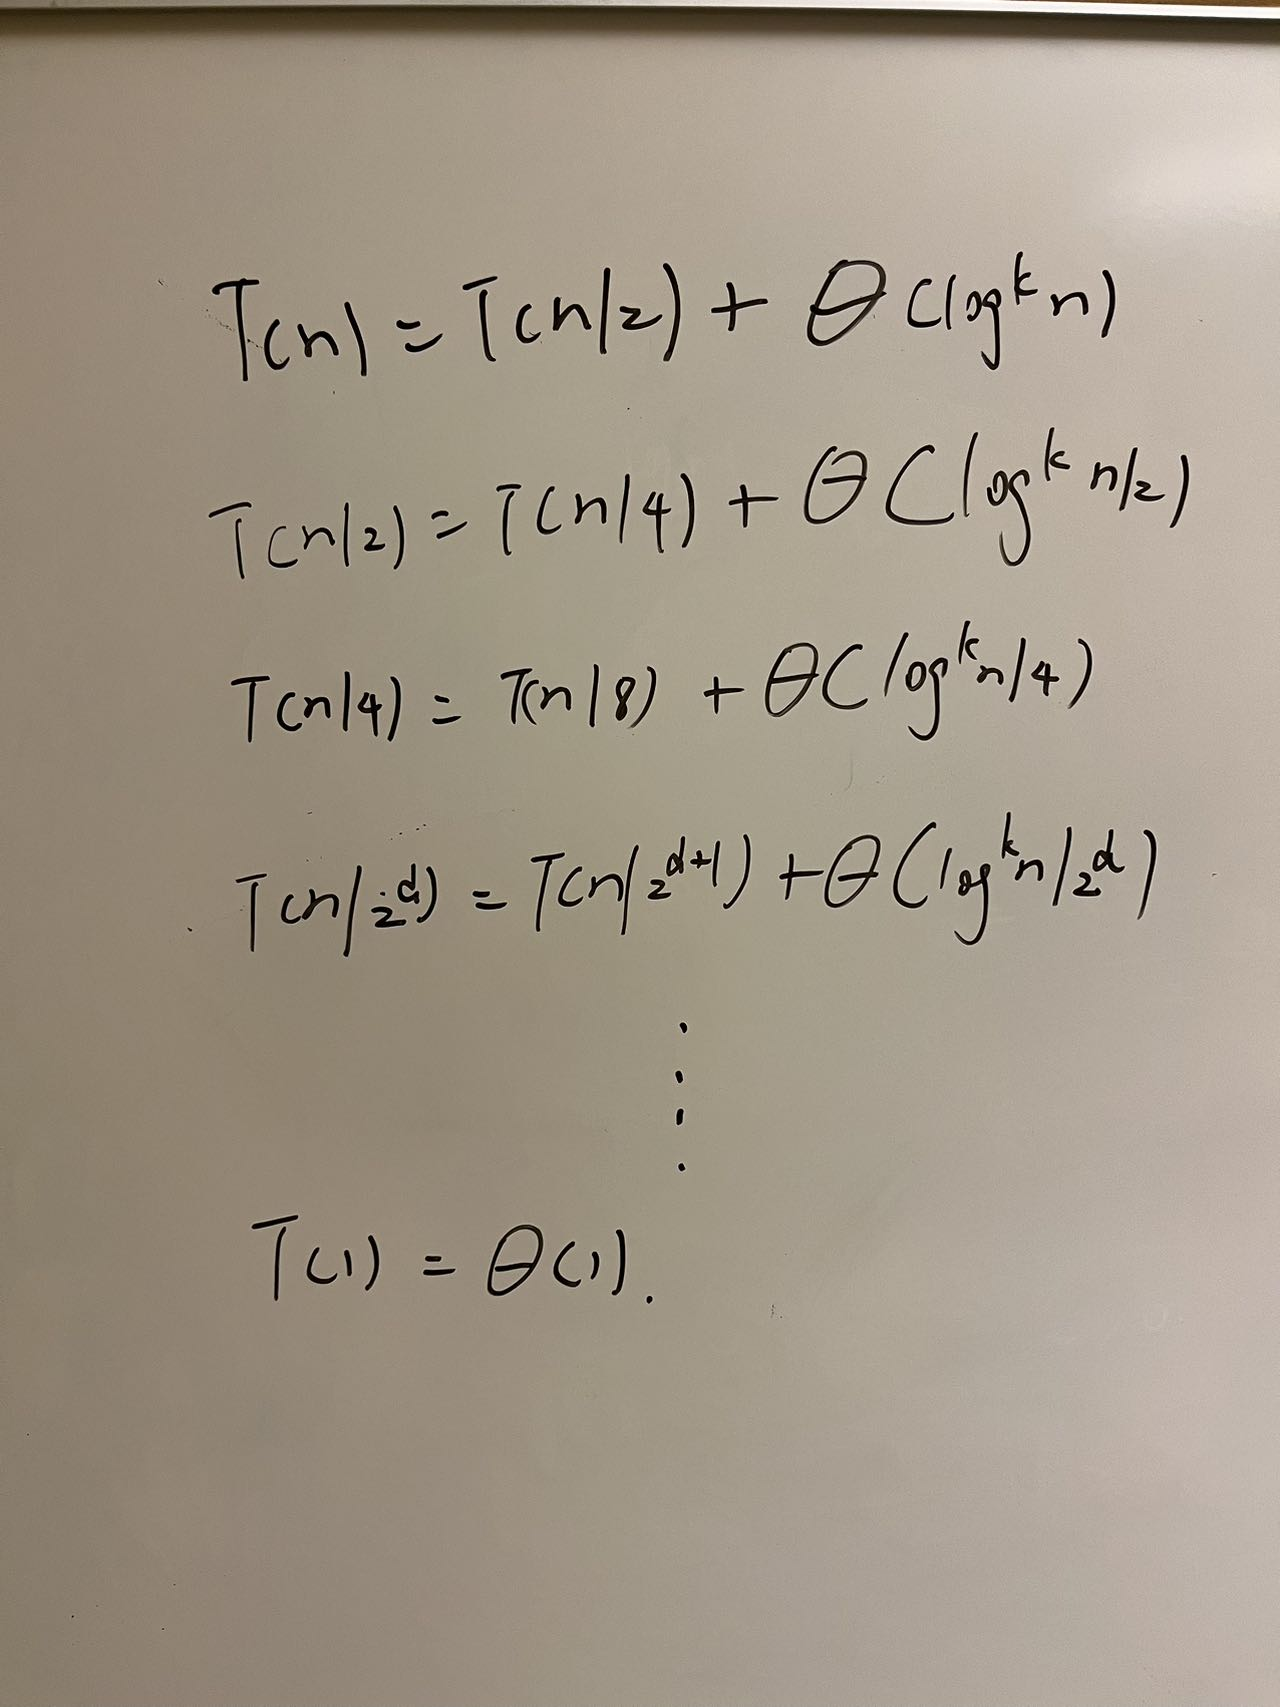
\includegraphics[scale = 0.13]{cool2.jpg}
\end{center}
From this substitution, there are total $L$ level which $n/2^L \rightarrow L = \log_2 n$.

We can then substitute $T(n/2), T(n/4) ,\dots$ and the expression for $T(n)$ will be:
\begin{align}
  \begin{split}
    T(n) &= T(n/2) + \Theta(\log^k n) \\
    T(n) &= T(n/4) + \Theta(\log^k n/2) + \Theta(\log^k n) \\ \nonumber
      &\vdots \\ \nonumber
    T(n) &= T(1) + \sum^{\log_2 n - 1}_{d=0} \Theta(\log^k n/2^d) \\ \nonumber
    T(n) &= \Theta(1) +\sum^{\log_2 n - 1}_{d=0} \Theta(\log^k n/2^d) \nonumber
  \end{split}
\end{align}
For the complexity, we can treat $\Theta(1)$ as constant, and for each element in $\sum^{\log_2 n - 1}_{d=0} \Theta(\log^k n/2^d)$,
Its time complexity will not exceed $O(\log^k n/2^d)$ and also not below $\Omega(\log^k n/2^d)$. This indicates that 
$$\sum^{\log_2 n - 1}_{d=0} c^\prime \cdot (\log^k n/2^d) \leq \sum^{\log_2 n - 1}_{d=0} \Theta(\log^k n/2^d) \leq \sum^{\log_2 n - 1}_{d=0} c \cdot (\log^k n/2^d) $$
where both $c$ and $c^\prime$ are constant. The equation also equals to:
$$c^\prime \sum^{\log_2 n -1}_{d=0}(\log_2 n - d)^k \leq \sum^{\log_2 n - 1}_{d=0} \Theta((\log_2 n - d)^k) \leq c \sum^{\log_2 n -1}_{d=0}(\log_2 n - d)^k$$
$$c^\prime \log_2^{k+1} n + c^\prime T \leq \sum^{\log_2 n - 1}_{d=0} \Theta((\log_2 n - d)^k) \leq c \log_2^{k+1} n + cT $$
where $T$ is the big chunk that does not contain $\log_2^{k+1} n$. Since the term with
biggest power will take the lead when $n$ grows very big, we can ignore the $T$ and the equation will become:
$$c^\prime \log_2^{k+1} n \leq \sum^{\log_2 n - 1}_{d=0} \Theta((\log_2 n - d)^k) \leq c \log_2^{k+1} n$$
$$\Omega(\log_2^{k+1} n) \leq \sum^{\log_2 n - 1}_{d=0} \Theta((\log_2 n - d)^k)  \leq O(\log_2^{k+1} n)$$
which means
$$\sum^{\log_2 n - 1}_{d=0} \Theta((\log_2 n - d)^k) = \Theta(\log_2^{k+1} n)$$
So
$$T(n) = \Theta(\log_2^{k+1} n)$$
$\blacksquare$



















$$c \cdot \sum^{\log_2 n -1}_{d=0}\log^k (n/2^d) + c^\prime $$
doing transformation for each addition part,
$$c \cdot \sum^{\log_2 n -1}_{d=0}(\log_2 n - \log_2 2^d)^k + c^\prime $$
\paragraph{Case 1:} Big-Oh \\
Since $\log_2 2^d = d$ and $d \geq 0$, $(\log_2 n - \log_2 2^d)^k$ will always smaller than $\log^k_2 n$.
This shows that 
\begin{align}
    c \cdot \sum^{\log_2 n -1}_{d=0}(\log_2 n - \log_2 2^d)^k + c^\prime &\leq c \cdot \sum^{\log_2 n -1}_{d=0}(\log_2 n)^k + c^\prime \\ \nonumber
    c \cdot \sum^{\log_2 n -1}_{d=0}\log^k (n/2^d) + c^\prime &\leq c \cdot \sum^{\log_2 n -1}_{d=0}(\log_2 n)^k + c^\prime \\ \nonumber
    &= c \cdot \log_2 n \cdot (\log_2 n)^k + c^\prime \\ \nonumber
    &= c \cdot \log^{k+1}_2 n + c^\prime \nonumber
\end{align}
Because $c$ and $c^\prime$ are both constant, let $g(n) =\log^{k+1}_2 n $, $f(n) =\sum^{\log_2 n -1}_{d=0}\log^k (n/2^d) + c^\prime$, if $c \textmd{,} N> 0$
$$f(n) \leq c \cdot g(n)$$
for all $n \geq N$, then 
$$f(n) = O(g(n)) = O(\log^{k+1}_2 n)$$










\section*{Question 3}
\subsection*{(a)}
The following is the pseudocode for this algorithm,
\begin{multicols}{2}
\begin{verbatim}
  function b = EXACT(S, a)
    if S = 0 
      return 1
    if size(a) = 0
      return 0
    end if
    init 2D-array dp[a+1][S+1]
    for i = 0:n-1 do
      dp[i][0] = 1
    end
    for i = 0:S-1 do
      dp[0][i] = 0
    end

    for i = 1:n do
      for j = 1:S do
        dp[i][j] = dp[i-1][j]
        if j >= a[i-1] and dp[i][j-a[i-1]] != 0
          dp[i][j] = 1
        end if
      end for
    end for

    return dp[a][S];
    end function
\end{verbatim}
\end{multicols}
\subsubsection*{Proof of Correctness}
\paragraph{}

For the base case when integer $S=0$, we can easily know that there exists a empty set which is the 
subset of the integers. For base case when size of nonnegative integers is $0$, we can also know that 
there is no subset which can add up to exactly $S$. So both base case is true.


For inductive process, the recurrence relation for $dp[i][j]$ will be,
$$dp[i][j] = \begin{cases}
  dp[i-1][j]\\
  dp[i-1][j-a[i-1]] & \text{if } dp[i][j-a[i-1]] \neq 0 \text{, } a[i-1] <= j
\end{cases}$$
Where $0$ indicates, no subset exists in current situation, and $1$ means there is a subset.


In case $dp[i][j] = dp[i-1][j]$, if $dp[i-1][j] = 1$, this means up to $a_{i-1}$,
a subset that satisfies the condition already exists. We can just pass that value to $dp[i][j]$.

If $dp[i-1][j] = 0$, this means up to $a_{i-1}$, there is no subset. We then have to check if adding
the current integer will create the subset. For condition $a[i-1] <= j$, we need to make sure the current
capacity is bigger than the integer we are checking or we can not add it anyway. The next step is for
$dp[i-1][j - a[i-1]]$. This entry means before adding the current integer, whether the subset for capacity $j-a[i-1]$ exists.
If it is true, we can just add the current integer and also increase the capacity.
Else, we will keep the number same as $dp[i-1][j]$. $\blacksquare$

\subsubsection*{Cost Analysis}
\paragraph{}
In my pseudocode, the initialization takes $O(n+S)$, and there is a nested loop which takes $O(nS)$.
Assume that comparison and assigning variables take constant time. The running time for my pseudocode will be $O(nS + n + S)$ where $n$ is the size of nonnegative set and
$S$ will be the nonnegative number. Because $nS$ takes the dominance, the running time will be,
$$O(nS)$$

The memory cost will also be $O(nS)$ because in my pseudocode, I create a table with size  $n \times S$. So the 
space complexity will be 
$$O(nS)$$


\subsection*{(b)}
When checking the existence, we find that all entries in one column only depends on the left one column.
Therefore, we can parallel each entry's calculations for every column.
The pseudocode for parallel will be,
\begin{multicols}{2}
  \begin{lstlisting}[mathescape=true]
    function b = EXACT(S, a)
      if S = 0 
        return 1
      if size(a) = 0
        return 0
      end if
      init 2D-array dp[a+1][S+1]
      for i = 0:n-1 do
        dp[i][0] = 1
      end
      for i = 0:S-1 do
        dp[0][i] = 0
      end
  
      for i = 1:n do
        $\textbf{parallel}$ for j = 1:S do
          dp[i][j] = dp[i-1][j]
          if j >= a[i-1]
            if dp[i-1][j-a[i-1]] != 0
              dp[i][j] = 1
            end if
          end if
        end for
      end for
      return dp[a][S];
      end function
  \end{lstlisting}
  \end{multicols}
  It is similiar to the code in section $(a)$, I just make the calculation for the inner loop become parallel.
  \subsubsection*{Correctness}
  
  The justification of correctness is also similiar. In this case, everything in previous proof also holds true.
  For each thread, it will be responsible for each entry and check whether $dp[i-1][j] = 1$. If not
  each thread will also check conditions $j >= a[i-1]$ and $dp[i-1][j-a[i-1]] != 0$. If these conditions are satisfied,
  $dp[i][j]$ will be labed as true.

  \subsubsection*{Work and Span}

  The work for this algorithm will be $T_1(n) = O(nS)$. For the span, since each thread can spawn new threads,
  The costs of spawning will be $O(\log S)$. The overal span will be $T_{\infty}(n) = O(n\log S)$.

  \subsubsection*{Parallelism}
  The parallelism $\overline{p}$ will be $$\frac{T_1(n)}{T_{\infty}(n)} = \frac{nS}{n\log S} =\frac{S}{\log S} $$
  which is representation of logrithmetic 







\end{document}